\section{Method}\label{6_method}
\begin{comment}
-- briefing
-- methods
-- pre-/post measurement
-- execution
-- interview
\end{comment}
\subsection{Conditions of Slackline Training}
Each participant is provided with the same levels, exercises, detailed description about the execution, and amount of training.
The difference in each conditions lies in the training method itself, how instructions are provided to the participant, and how feedback about the execution is given. All participants agreed to train without shoes but with socks to provide a consistent training condition per participant.
In the following each condition is described as well as its apparatus.

\subsubsection{Interactive System Group (ISG)}
Within the ISG condition two participant had no experience with interactive devices, four had intermediate experience or advanced experience.

The participant interacts on her own with the system, which teaches the user how to interact with it and guides her through predefined exercises.
It explains the user how to execute the exercises with a step by step description and a looping video of the correct execution.
Furthermore, how many repetitions and in which time to accomplish each repetition.
It provides real-time feedback about the current execution performance with several indicators.
Since it is a think-aloud study, the participant further tells on which actions she is troubling with and when there is any confusion or misunderstanding with the system implementation.
The experiment leader had no influence about questions regarding the exercise execution to ensure the autonomy of the user with the system.

\subsubsection{Human Trainer Group (HTG)}
The participant is instructed by a human trainer, which is the director of the study.
At first the trainer provides an instruction about the ongoing level of exercises.
Then the specific exercise is instructed on how to execute the exercise, how many repetitions, and the minimum time the trainee should hold the pose.
After that the trainer demonstrates the execution of the exercise for the trainee.
The trainer himself has an exercise description sheet to provide the trainee with the same information as the ISG.

\begin{figure}[htb]
	\centering
	\begin{minipage}[t]{1\linewidth}
		\centering
		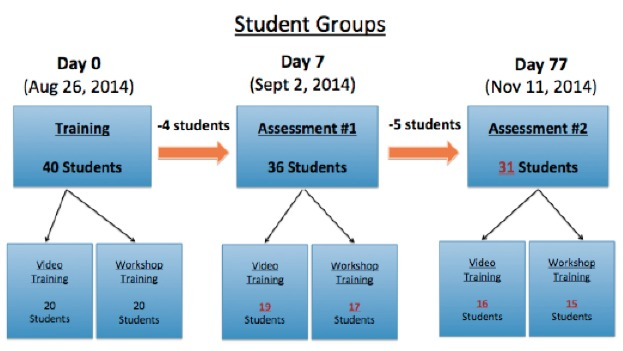
\includegraphics[width=0.8\linewidth]{Pictures/6_studyGroupsExample}
		\caption{Study groups example}
		\label{fig:6_studyGroups}
	\end{minipage}
\end{figure}

\subsection{Procedure}
At first the participant was welcomed and briefed about the idea as well as what she can expect from the study.
Further an introduction about the training method in which she participates was given.
After agreeing to participate on the study she had to confirm a form consent.
Next she had to answer a questionnaire for collecting demographic data and her prior experience with slacklining.
The ISG had to answer one more question about the prior experience with interactive devices (e.g. Kinect, Wii, PlayStation Move, etc.).
%Therefore one can see if a person, which tends to have a better experience with the system during the study, relies on her prior experience with such devices. 
The physical activity level as well as the lateral preference was determined like stated above.

At first the general balance ability of the participant was obtained before pre-measurement to exclude participants with a balance disorder.
Thereby she had to execute a single leg stand for the right and the left foot at first on the ground and then on a towel for a maximum of 10 seconds with 3 trials.
This ensures the participant has no problems with holding her own balance on a stable as well as on a uneven underground.

\todo{as few steps as possible to have a comparison}
After successful accomplishment the actual pre-measurement test was conducted.
It is divided in two parts.
First, a single leg stance for the left and right foot on the slackline with a maximum of 10 seconds.
Second, trying to walk on the entire slackline with the left as well as the right leg as starting point.
For each measurement and leg the participant had to accomplish three trials, which results in an amount of 12 trials.

After finishing the pre-measurements the participant was again shortly introduced about the ongoing procedure.
For all exercises she had to stay on a marked position at the ground, which visualizes the starting point.
Depending on the training method, the introduction, repetitions and time to hold each exercises is provided by the trainer or interactive system.
During the execution either the trainer or the system hints the participant about the correct execution of the exercise.
If an execution was not accurate, she had to repeat it until all repetitions of the exercises are accomplished successfully.
The participant had the possibility to skip the exercise if it was too difficult to accomplish or not appropriately recognised by the system.
During the training she could take breaks if she wanted to.
When accomplishing an exercise set, the participant was asked to rank the exercise she just completed on a scale of 1 (very easy) to 5 (very difficult).
%Therefore the ranking of the participant can be compared with the logged performance data.
%Hereby, it can be shown if the difficulty of the exercise set in each level is increasing and match the users' assumptions. %integrated exercise routine.

After finishing the training part a post-measurement was conducted with the same procedure as in the pre-measurement seen above.

Finally the participant had to answer questions in a semi-structured interview to obtain her opinion on the general training method and application scenarios for exactly this method with the slackline and other sport activities that could fit this method.
The ISG were additionally asked about the user interface of the slackline learning system and their experience with the interaction.
The specific questionnaires and interview questions can be seen in \todo{Appendix}.
%for reviewing and validating performance parameters as well as to detect system failures.

\subsubsection{Apparatus}
Figure \todo{[figure]} shows the setup of the study.
The Kinect was attached on a tripod with a height of \todo{90 cm}.
It is placed in front of a wall, which is used as projector screen.
The camera is faced in the direction of the slackline.
A projector is mounted on the ceiling of the room to project the systems interface on a wall.
The mobile slackline stands, like discussed in Section~\ref{5_1_hardwareComponents}, directly in front of the Kinect.
Marker attached on the slackline provide information for pre- and post-measurements as well as the starting point for the participant to get up the line.
The set up for the human trainer group was the same, but without the projector and the Kinect.
To record the execution a video camera was placed behind the participant to have her actions as well as the interface interaction recorded.
The set up was not changed during the study to have the same condition for every participant.

\todo{[Figure]}


\subsection{Design and independent \& dependent variables}\label{6_variables}
The experiment of the study is a 2 x 2 mixed factorial design, more specifically a 2 levels of group (group: ISG, HTG)  x 2 measurements (time: pre, post).
%Subjects were randomly assigned to a interactive system group (ISG) or a human trainer group (HTG).
Within subject a pre-measurement and post-measurement after the training was conducted.
The measurements are divided into three parts.
First, measuring the time of a single leg stance with the left as well as the right foot on the slackline with a stopwatch by the director of the study.
Second and third, measuring the steps and distance the participant can walk on the slackline with the left and right foot as starting point.
Therefore the slackline was divided into 12 parts with tape marks with a distance of 0.5 meters for each, to be able to measure the distance on the video recording with a certain amount of accuracy.
Three consecutive attempts per side of the foot and method were executed and measured to compare the results.
All pre- and post-measurement were recorded by video.
With the help of these video recordings each trial of the participants were checked twice after the study.

\textbf{Independent variables}
\begin{itemize}
\item Interactive Slackline Group
\item Human Trainer Group
\end{itemize}

\textbf{Dependent variables}
\begin{itemize}
\item Time stood on line with left and right foot
\item As many steps as possible on the line 
\item Walking as far as possible on the line
\end{itemize}

%The time was counted if the balancing leg of the participants leaves the ground and stopped if she gets in contact with the ground with any foot.


%\textbf{Confounding variable}
%\begin{itemize}
%\item Experience with general balance training
%\item Experience with slacklining
%\item General physical activity
%\end{itemize}

%A measurement of the participants' current balance performance was conducted before and after the training to compare the training results and learning progress.  This involves the measurement of how long the participant can stand on the slackline in seconds with her left, right, and with both feet. Further, how many steps were she able to walk on the slackline with the left or right foot for getting up the line. Three attempts per side and method were executed and \todo{the best taken / the average calculated} to compare the results.

% https://explorable.com/pretest-posttest-designs --> The Two Group Control Group Design


\begin{comment}
2 x 2 mixed factorial design
2 within subject --> test
pre-test
post-test

2 between subject --> training
Experiemental group --> ISG
Base line group --> HTG

ODER

3 dependent vs 2 independent variables
\end{comment}